\documentclass[a4paper,
               %boxit,
               %titlepage,   % separate title page
               %refpage      % separate references
              ]{jacow}

\ifboolexpr{bool{xetex} or bool{luatex}} % test for XeTeX/LuaTeX
 {}                                      % input encoding is utf8 by default
 {\usepackage[utf8]{inputenc}}           % switch to utf8

\usepackage{graphicx, subfigure}
\usepackage{booktabs}


\begin{document}
\title{BEAM COUPLING IMPEDANCE OF THE NEW BEAM SCREEN OF THE LHC INJECTION KICKER MAGNETS}
\author{H. Day\thanks{hugo.day@hep.manchester.ac.uk}$^{\dagger}$, M.J. Barnes$^{\dagger}$, F. Caspers$^{\dagger}$, E. Métral$^{\dagger}$, B. Salvant$^{\dagger}$ \\
$\dagger$ CERN, Switzerland
}

\maketitle 


\begin{abstract}
The LHC injection kicker magnets experienced significant beam induced heating of the ferrite yoke, with high intensity beam circulating for many hours, during operation of the LHC in 2011 and 2012. The causes of this beam coupling impedance were studied in depth and an improved beam screen implemented to reduce the impedance. Results of measurements and simulations of the new beam screen design are presented in this paper: these are used to predict power loss and temperature of the ferrite yoke for operation after long shutdown 1 and for proposed HL-LHC operational parameters.
\end{abstract}

\section{Introduction}

\section{New Design}

\section{Impedance Measurements}

\section{Power Loss and Future Improvements}
%Title format - Title; Authors; Affiliation; conference
%Abstract - Copied from submitted abstract (maybe changed to represent changes in presented paper)
%Introduction
%Body of data
%Conclusion
%Acknowledgements
%References

% Aim of paper - To present the causes of the beam coupling impedance in the beam screen - length of overlap, thickness, screening by conductors. Expected power loss for the new screen design with present and HL-LHC parameters
% Sections:
% Introduction - Brief history of the MKI heating - reference to Mike's paper last year and this year
% Reasons for the impedance - Distinction between well screened and not well screened
% - Increasing number of screen conductors reduces effect of the ferrite
% - Dimensions of the capacitive end changing impedance profile
% - Effect of different ferrites on the 30-40MHz peak if time
% Power loss expectactions for HL-LHC, post LS1 between 15, 19 and New design
%
%
%

% Images to include
% New screen design cross section
% New screen design impedance
% Various lengths of overlap impedance and predicted resonant frequency
% 

\section{INTRODUCTION}

During the 2011 and 2012 runs of the LHC, high temperatures were observed in several devices in the LHC  \cite{metral_cham2012}, a critical piece being the LHC injection kicker magnets (MKIs, Fig.~\ref{fig:mkiStruct}), which were attributed to beam-induced heating due to high power loss from the interaction of the circulating beam with the longitudinal beam coupling impedance. This heating was observed to raise the temperature of the ferrite yoke of one of the MKIs above its Curie point during fills, thereby necessitating waiting times of several hours for the ferrite to cool before safe injection could be carried out \cite{mki-heating}. 

In response to this an extensive study to reduce the temperature of the ferrite yoke was carried out, aimed at reducing the power loss into the kicker magnet and increasing the transfer of thermal energy from the ferrite yoke to the surroundings \cite{mki-heatingTemp}. A new beam screen was implemented in MKI8D in technical stop 3 (TS3) (23/09/12-27/09/12) with improved screening of the ferrite from the beam and some modifications to reduce the likelihood of electrical breakdown during magnet pulsing: this was observed to greatly reduce the temperature of the ferrite yoke \cite{mki-heatingTemp}. Building on this success, further modifications to the beam screen have been proposed to further reduce the beam coupling impedance. In addition, the reasons for the resulting impedance in a well screened magnet (i.e. where the beam does not see the ferrite yoke) are discussed. 

\begin{figure}
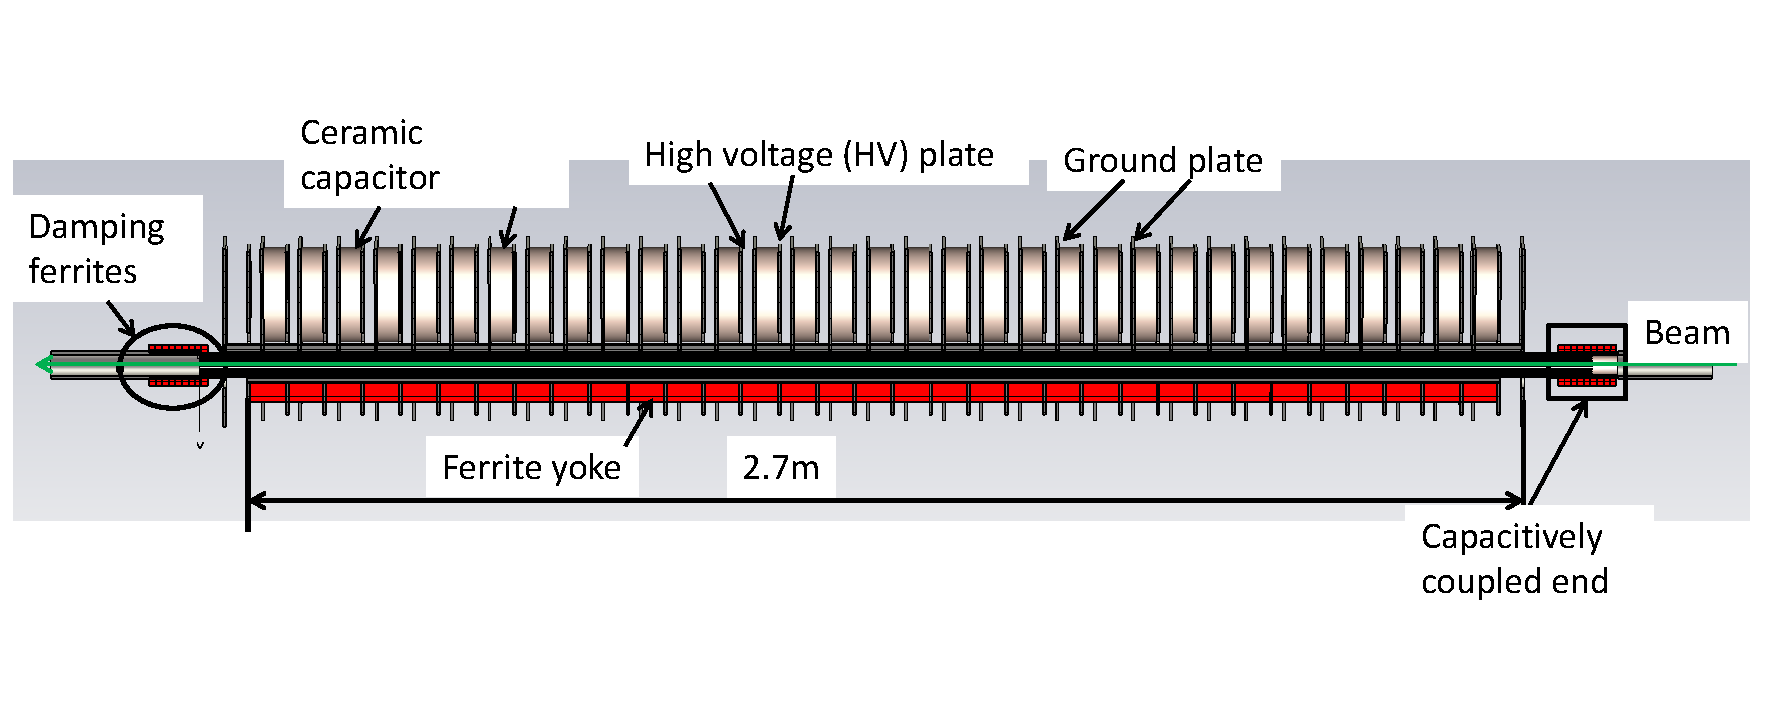
\includegraphics[width=0.5\textwidth]{MKICrossSectionYZ.pdf}
\caption{Structure of the injection kicker magnets.}
\label{fig:mkiStruct}
\end{figure}



\begin{thebibliography}{9}
\bibitem{metral_cham2012}
E. Métral \emph{et al}., \emph{Beam-Induced Heating/Bunch Length/RF and Lessons for 2012}, LHC Performance Workshop, Chamonix 2012, CERN-ATS-2012-069. 

\bibitem{mki-heating}
M.J. Barnes \emph{et al}., \emph{"Analysis of Measured Ferrite Heating of the LHC Injection Kickers and Proposals for Future Reduction of Temperature"}, IPAC'12, New Orleans, USA, 2012, TUPPR090.

\bibitem{mki-heatingTemp}
M.J. Barnes \emph{et al}., \emph{"Beam Induced Ferrite Heating of the LHC Injection Kickers and Proposals for Improved Cooling"}, IPAC'13, Shanghai, China, MOPWA031.

\bibitem{kicker_meas}
H. Day \emph{et al}., \emph{"Evaluation of the Beam Coupling Impedance of new Beam Screen Designs for the LHC Injection Kicker Magnets"}, IPAC'12, New Orleans, USA, 2012, WEPPR071.

\bibitem{mki-ElecBreakdown}
M.J. Barnes \emph{et al}., \emph{"Reduction of Surface Flashover of the Beam Screen of the LHC Injection Kickers"}, IPAC'13, Shanghai, China,, MOPWA031.

\bibitem{cst-cite}
\texttt{http://www.cst.com}.

\bibitem{DayThesis}
PhD Thesis, H. Day, 2013.

\bibitem{LHCRF}
P. Baudrenghien \emph{et al}., \emph{"The LHC RF System - Experience with Beam Operation"}, IPAC'11, San Sebastian, 2011, MOPC054.


\end{thebibliography}
\end{document}

